\documentclass[10pt,twocolumn]{article}

\usepackage[a4paper,margin=17mm,columnsep=7mm]{geometry}
\usepackage[T1]{fontenc}
\usepackage[utf8]{inputenc}
\usepackage{lmodern}
\usepackage{microtype}
\usepackage{booktabs}
\usepackage{array}
\usepackage{amsmath}
\usepackage{graphicx}
\usepackage{tikz}
\usetikzlibrary{arrows.meta,positioning,fit,calc,shapes.geometric}
\usepackage{xcolor}
\usepackage[hidelinks]{hyperref}
\usepackage{enumitem}

\definecolor{accent}{HTML}{174A7E}
\setlength{\parindent}{1em}
\setlength{\parskip}{0pt}
\setlength{\columnsep}{7mm}
\setlist{nosep,leftmargin=*}
\renewcommand{\arraystretch}{1.06}
\newcommand{\todo}[1]{\textcolor{red!70!black}{[FINAL MEASUREMENT: #1]}}

\title{\vspace{-1.5em}
\resizebox{0.98\textwidth}{!}{\textbf{How I Beat the Throughput of a Popular C++ Order Book by 4$\times$}}\\[-0.05em]
\normalsize An independently implemented, cache-aware C++ limit order book with constant-time cancellation}
\author{\normalsize \todo{author name and GitHub URL}}
\date{}

\begin{document}
\fontsize{9.5}{11.2}\selectfont
\maketitle
\vspace{-1.4em}

\begin{abstract}
This report describes the design, implementation, and evaluation of \textit{babobook}, a
single-threaded limit order book written independently in C++.  The
implementation follows the theoretical direction of Yoon's
Priority-Indicated Node (PIN) architecture~\cite{yoon2026}, but the order-book core, tree, node,
memory, and order-lifecycle code presented here are my own.  I compare \textit{babobook}
with \textit{Liquibook}, a well-known open-source C++ order-book implementation, behind one
C ABI and on identical deterministic workloads.  On the representative
simulated workload, the final experiment targets the paper's headline of
approximately 4$\times$ throughput; in a deliberately static, cancellation-heavy
stress case, the saved harness run already shows a 79.7$\times$ difference.  The
large static gap exposes the mechanism rather than standing in for normal
market traffic: \textit{Liquibook} scans a per-price container to locate a cancellation,
whereas \textit{babobook} maps an order identifier directly to a stable slot.  Performance
is accepted only after the complete report stream matches a trusted SHA-256
reference and the order book passes live state queries at unpredictable replay
positions.
\end{abstract}

\section{Introduction}

An electronic limit order book receives a totally ordered stream of messages,
maintains bids and asks, preserves price--time priority, and determines
executions.  For one instrument this state transition is inherently
serial: sharding the surrounding gateway does not remove the single-writer
dependency inside the book.  During a traffic burst, if orders arrive faster
than the book can process them, unprocessed messages wait upstream and latency
increases.  The book's sustainable throughput determines when that backlog
begins to form.

This makes an order book a useful low-latency systems case study.  It combines an
ordered price index, FIFO priority within each price, arbitrary cancellation by
identifier, multi-level matching, and deterministic output.  It also punishes
designs whose asymptotic behavior looks acceptable until cache misses,
allocation, or a dominant linear scan appears in the hot path.

I built \textit{babobook} to investigate that interaction.  I used the public workload and
benchmark contract released with Yoon's paper~\cite{yoon2026} as a starting point, then
independently implemented the order book and its data
structures.  The comparison in this report asks a deliberately narrow question:
given the same valid order stream and the same observable output contract, how
much throughput can a cache-aware, direct-cancel design sustain relative to the
vendored \textit{Liquibook} baseline?

The contributions of the project are:
\begin{itemize}
  \item an independently written order-book core supporting limit, IOC, AON,
        stop, cancel, modify, and market-price behavior;
  \item fixed-capacity inline order nodes with stable slots and O(1) unlinking;
  \item an order-id index that turns arbitrary resting-order cancellation into
        a direct lookup and erase;
  \item a threaded, per-side price-level tree with best-first traversal;
  \item pull-based aggregate depth, derived from the tree rather than updated in
        a separate ordered container on every operation;
  \item a cross-platform C-ABI harness with full-stream correctness hashing and
        an independent state audit; and
  \item adapters and a documented template through which another order book can be
        evaluated under the same contract.
\end{itemize}

This is an engineering report, not a claim of novel theory or a production-ready
exchange matching engine.  Networking, persistence, recovery, risk, regulatory controls, and
multi-symbol scheduling are outside the timed system.  The result applies to the
specified code revisions, workloads, compiler, and hardware; it does not imply
that every conventional order book has the same cancellation behavior as
\textit{Liquibook}.

\section{Order-book operations and the bottleneck}

\subsection{A minimal order-book vocabulary}

An order book is a live collection of intentions to buy and sell.  A \emph{bid}
offers to buy a quantity at a stated price; an \emph{ask} offers to sell.  The
highest resting bid is the \emph{best bid}, the lowest resting ask is the
\emph{best ask}, and the gap between them is the \emph{spread}.  An incoming
order crosses the spread when a buyer is willing to pay at least the best ask,
or a seller is willing to accept at most the best bid.  The resting order is the
\emph{maker}; the incoming order that removes liquidity is the \emph{taker}.

The bid side ranks higher prices first; the ask side ranks lower prices first.
Within one price, earlier orders execute first.  A useful representation must
therefore support two related orderings: a dynamic ordered set of prices and a
FIFO sequence of orders at every price.

The project supports several common order instructions:
\begin{itemize}
  \item A \textbf{limit order} trades only at its limit price or a better one.
        Any unmatched remainder can rest in the book.
  \item A \textbf{market order} prioritizes immediate execution and consumes the
        best available opposite orders until filled or the opposite side is
        empty.
  \item \textbf{IOC} (Immediate or Cancel) matches immediately, then cancels any
        quantity that could not execute.  An IOC remainder never becomes a
        resting order.
  \item \textbf{AON} (All or None) may execute only if its entire remaining
        quantity is available under its price constraint; otherwise it waits or
        remains unexecuted rather than taking a partial fill.
  \item \textbf{FOK} (Fill or Kill) combines AON and IOC: fill the entire order
        immediately or cancel it without a partial execution.
  \item A \textbf{stop order} remains parked outside the active bid/ask book
        until the observed market price reaches its trigger, after which it is
        submitted for normal processing.
  \item A \textbf{modify} changes a resting order.  In the benchmark contract it
        is deliberately defined as cancel plus reinsert, so the order loses its
        previous time priority.
\end{itemize}

\begin{figure*}[t]
\centering
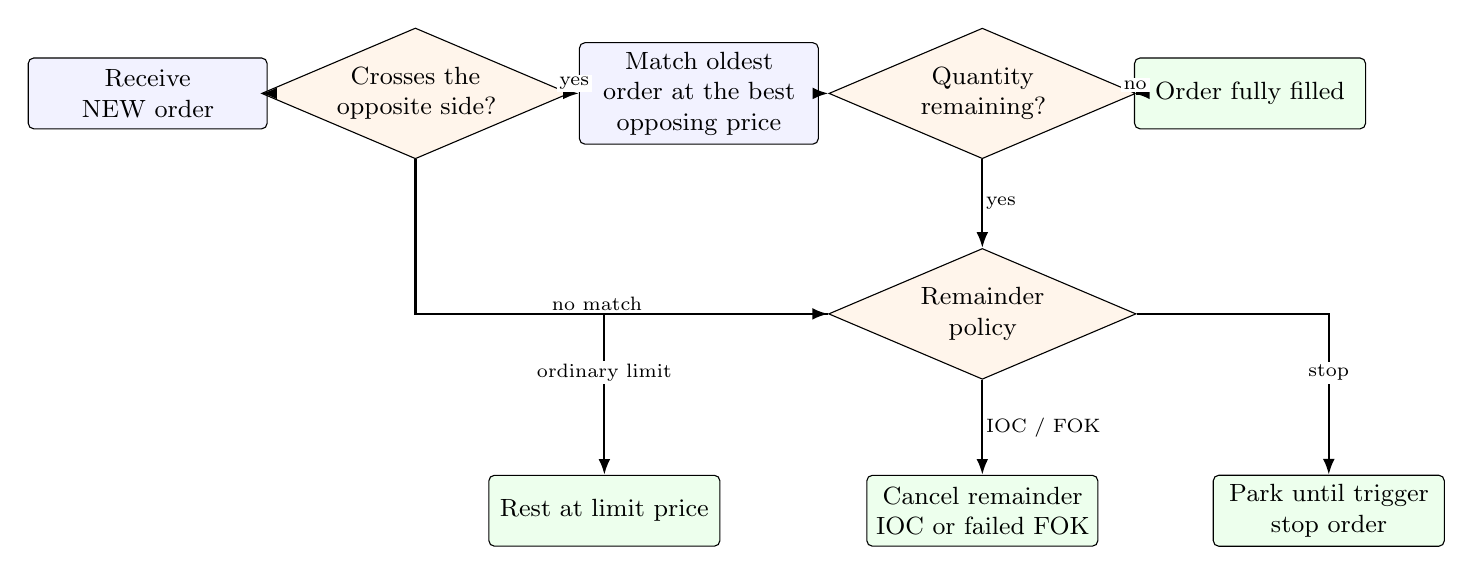
\begin{tikzpicture}[
  font=\small,
  box/.style={draw,rounded corners=2pt,minimum height=9mm,text width=28mm,align=center,fill=blue!5},
  decision/.style={draw,diamond,aspect=2.35,minimum height=12mm,text width=21mm,align=center,fill=orange!8,inner sep=1pt},
  outcome/.style={draw,rounded corners=2pt,minimum height=9mm,text width=27mm,align=center,fill=green!7},
  arrow/.style={-{Latex[length=2mm]},thick},
  edgeword/.style={font=\scriptsize,fill=white,inner sep=1pt}
]
\node[box] (new) at (0,0) {Receive NEW order};
\node[decision] (cross) at (3.4,0) {Crosses the opposite side?};
\node[box] (match) at (7.0,0) {Match oldest order at the best opposing price};
\node[decision] (remaining) at (10.6,0) {Quantity remaining?};
\node[outcome] (filled) at (14.0,0) {Order fully filled};
\node[decision] (policy) at (10.6,-2.8) {Remainder policy};
\node[outcome] (rest) at (5.8,-5.3) {Rest at limit price};
\node[outcome] (cancel) at (10.6,-5.3) {Cancel remainder\\IOC or failed FOK};
\node[outcome] (park) at (15.0,-5.3) {Park until trigger\\stop order};

\draw[arrow] (new) -- (cross);
\draw[arrow] (cross) -- node[edgeword,above]{yes} (match);
\draw[arrow] (match) -- (remaining);
\draw[arrow] (remaining) -- node[edgeword,above]{no} (filled);
\draw[arrow] (remaining) -- node[edgeword,right]{yes} (policy);
\draw[arrow] (cross.south) |- node[edgeword,pos=.72,above]{no match} (policy.west);
\draw[arrow] (policy) -| node[edgeword,pos=.72,above]{ordinary limit} (rest.north);
\draw[arrow] (policy) -- node[edgeword,right]{IOC / FOK} (cancel);
\draw[arrow] (policy) -| node[edgeword,pos=.72,above]{stop} (park.north);
\end{tikzpicture}
\caption{Reader-level order lifecycle. AON/FOK perform an all-or-nothing
quantity check before allowing partial execution; IOC prevents any unfilled
remainder from resting.}
\label{fig:order-lifecycle}
\end{figure*}


For an incoming order, the order-book core repeatedly inspects the best opposite price.
If the prices cross, it trades against the oldest maker at that price, updates
quantities, removes filled orders and empty levels, and continues until the
incoming quantity is exhausted or no longer crosses.  A non-IOC residual rests
on its own side.  A modify in the benchmark is cancel plus reinsert, and thus
loses time priority.  Every command emits a deterministic acknowledgement,
trade, or rejection sequence.

The target costs are shown in Table~\ref{tab:costs}.  The important distinction
is between finding an order and unlinking an order.  An intrusive list can unlink
a known node in O(1), but a cancellation is still linear if the implementation first
walks a price-level container to discover that node.

\begin{table}[h]
\centering
\caption{Target operation costs.}
\label{tab:costs}
\small
\begin{tabular}{@{}ll@{}}
\toprule
Operation & Target cost \\
\midrule
Order lookup by id & O(1) average \\
Cancel known resting order & O(1) \\
Locate arbitrary price level & O($\log P$) \\
Best/near-best price discovery & O(1) fast path \\
Append after level is located & O(1) \\
Consume best maker & O(1) per fill \\
Create/remove price level & O($\log P$) rebalance \\
Advance to adjacent price & O(1) \\
Build top-$N$ depth snapshot & O($N$) per query \\
\bottomrule
\end{tabular}
\end{table}

Here $P$ is the number of active price levels on one side.  The O(1) append
claim begins only after the target level is known; it does not imply that every
price lookup is constant-time.  The implementation avoids a general tree walk
for the common local cases: the order is at the current best price, improves the
best price, hits the immediate worse neighbor, falls between the best and that
neighbor, or extends a single-level book.  An arbitrary deeper price uses the
balanced-tree search path, giving O($\log P$) discovery before the fixed-slot
append.  This separation between \emph{locating a price level} and \emph{placing
an order into that level} is important when interpreting the design's costs.

\subsection{Why the baseline slows down}

\textit{Liquibook} is not an obscure implementation selected only because it is
easy to beat.  Its public repository describes it as a ``Modern C++ order
matching engine'' and, as observed on 11 July 2026, reports approximately 1.5k
stars, 436 forks, and 128 watchers~\cite{liquibook}.  GitHub popularity does not
prove that its architecture represents every production venue, but it makes
Liquibook a recognizable, independently available baseline whose source,
license, tests, and native performance program readers can inspect directly.

\textit{Liquibook} stores each side of the resting book in a
\texttt{std::multimap<ComparablePrice, Tracker>}.  The container efficiently
finds the first entry for a price, but the evaluated cancel and modify paths
still call \texttt{find\_on\_market()}, which walks forward through the
equal-price entries and compares order pointers until it finds the requested
order.  The comparison is therefore not a claim that \texttt{std::multimap}
itself is always linear: the measured scaling cost is Liquibook's identity
lookup among the orders sharing that price.  As many orders accumulate around
a small set of prices, the amount of work per cancel grows.  Babobook instead
uses its order-id index to reach the owning PIN and slot directly.  This
difference is especially costly for the baseline in the supplied workload
because 95\% of eligible resting orders later receive cancellation requests.

The static scenario intentionally holds the midpoint fixed.  It concentrates
orders into deeper queues and exposes this scaling difference.  It is not the
representative headline workload; it is the diagnostic experiment that makes
the O($n$) versus O(1) mechanism visible.

Complexity alone is not the entire story.  A node-per-order linked structure
also scatters payloads, creates dependent pointer loads, and frustrates hardware
prefetch.  A single flat array has good locality but makes arbitrary deletion
expensive if elements must move.  The design challenge is to retain stable,
directly addressable locations without surrendering locality.

\subsection{Why this design fits real order flow}

The design is aimed at the shape of real electronic order flow, not at a uniform
random key-value workload.  Published order-book studies report that placement
and update activity are concentrated near the best bid and ask, with activity
falling away from the touch but retaining a long tail~\cite{gould2013,cont2010}.
The reference paper additionally motivates the design with cancel-dominated
traffic---approximately 95\% of submitted orders are cancelled rather than
executed---and with short, intense market micro-bursts~\cite{yoon2026}.  The
benchmark generator encodes these characteristics through a 95\% cancellation
probability, sub-millisecond median lifetime, a near-touch liquidity hump, and a
power-law depth tail.

This distribution creates a small hot region and a much larger cold region.
Orders close to the prevailing price are inserted, modified, matched, and
cancelled repeatedly, while deeper orders are touched less often and remain in
the book longer.  A cache-friendly representation benefits twice: contiguous
hot nodes improve spatial locality and prefetching near the touch, while stable
slots and the direct order-id index avoid scanning or compacting a queue when a
cancellation targets an arbitrary resting order.  Fixed-capacity nodes also
bound the amount of memory pulled into cache for one operation instead of
following a long chain of separately allocated objects.

These properties make the architecture suitable for realistic cancellation-heavy
workloads, but they do not make every result a measurement of a live venue.  The
current scenarios are deterministic synthetic workloads calibrated to documented
market characteristics.  That distinction lets the experiment preserve valid
order identities and exact reproducibility while remaining explicit about what
``realistic'' means.

\section{Implementation}

\subsection{Fixed-slot priority nodes}

The basic storage unit is \texttt{pin\_node<N>}, a fixed-capacity region of
inline order slots.  Live slots are connected by intrusive previous/next slot
indices that encode logical priority independently of physical position.  A
node also links to adjacent nodes in the global priority chain.  Insertion takes
a free slot and updates a bounded number of indices; erasure unlinks the slot
and returns it to the node's free list.  Existing payloads do not move during a
normal cancellation.

The physical representation is deliberately simple enough to reconstruct.  A
node contains four categories of state:
\begin{itemize}
  \item \texttt{slots[N]} is an inline array of complete order values.  Slot
        address is always \texttt{base + index * sizeof(order)}.
  \item \texttt{links[N]} stores two 16-bit indices per slot.  For a live slot,
        \texttt{prev} and \texttt{next} form the node-local priority list.  For a
        free slot, \texttt{next} is reused as the node's free-list pointer.
  \item \texttt{head}, \texttt{tail}, \texttt{free}, and \texttt{size} describe
        the first/last live slot, first reusable slot, and current occupancy.
        The all-ones 16-bit value is the null index.
  \item \texttt{prev\_node} and \texttt{next\_node} link this fixed-capacity
        region into the side's global PIN chain.
\end{itemize}
Construction threads every slot into the free list.  Allocation pops one index,
moves or assigns the order into that slot, and increments \texttt{size}.  The
three primitive insertions then perform only local link writes:
\texttt{prepend} makes the slot the node head; \texttt{append} makes it the node
tail; and \texttt{insert\_after(ref)} splices it between \texttt{ref} and the
old successor.  Erase performs the symmetric operation, fixes head or tail when
needed, and pushes the slot index back onto the free list.  It neither shifts a
suffix nor compacts the array; the stale payload is simply overwritten on reuse.

The key invariant is therefore \emph{stable physical slot, mutable logical
priority}.  Slot 3 may precede slot 0, which may precede slot 11.  Priority comes
from the small link indices, not array position.  This is what combines
contiguous storage with arbitrary O(1) unlinking.

If the target node is full, the tree performs a bounded, directed relocation
cascade toward a node with capacity.  Each hop moves one boundary order and
updates its recorded location.  A new pooled node is linked at the boundary if
no free slot is reached within the configured hop limit.  Node capacity is a
compile-time parameter; the repository can build capacities 16, 32, 64, and 128
for an empirical cache-locality sweep.  In the measured workloads this sweep
did not produce a meaningful throughput difference: results across the tested
capacities remained within ordinary run-to-run variation.  Node capacity is
therefore reported as a robustness check rather than presented as a tuned source
of the headline speedup.

\subsection{The global PIN chain}

PIN nodes are not owned independently by price levels.  For each book side,
\textit{babobook} maintains one global doubly linked chain of PIN nodes ordered
from the globally best order to the globally worst order.  Within each PIN node,
intrusive slot indices encode the same logical sequence.  Advancing through all
orders therefore means following an intra-node slot link and, only at a node
boundary, moving to the head slot of the next PIN node.  This realizes the
paper's global PIN-chain organization~\cite{yoon2026} while retaining fixed,
contiguously addressable storage inside every node.

Orders belonging to one price form a contiguous logical sub-range of this global
chain.  The corresponding price-level descriptor does not own a separate list
or PIN node.  Instead, it stores two \texttt{order\_loc} values: \texttt{\_head}
points to the highest-priority order at that price and \texttt{\_tail} points to
the newest, lowest-priority order at that price.  Each location is the pair
\{PIN-node pointer, slot index\}.  The descriptor also stores aggregate open
quantity and resting-order count, so tree traversal can answer depth queries
without walking the orders in its sub-range.

This separation is important.  The NARB Tree answers \emph{which price level}
is next; the global PIN chain answers \emph{which order} is next under complete
price--time priority.  A new order at an existing level is inserted immediately
after that descriptor's tail.  A newly created price level is inserted after the
tail of its immediately better neighboring level, or at the global chain head if
it becomes the new best.  Consequently, price-level boundaries remain explicit
even when one physical PIN node contains slots belonging to more than one price.

\begin{figure*}[t]
\centering
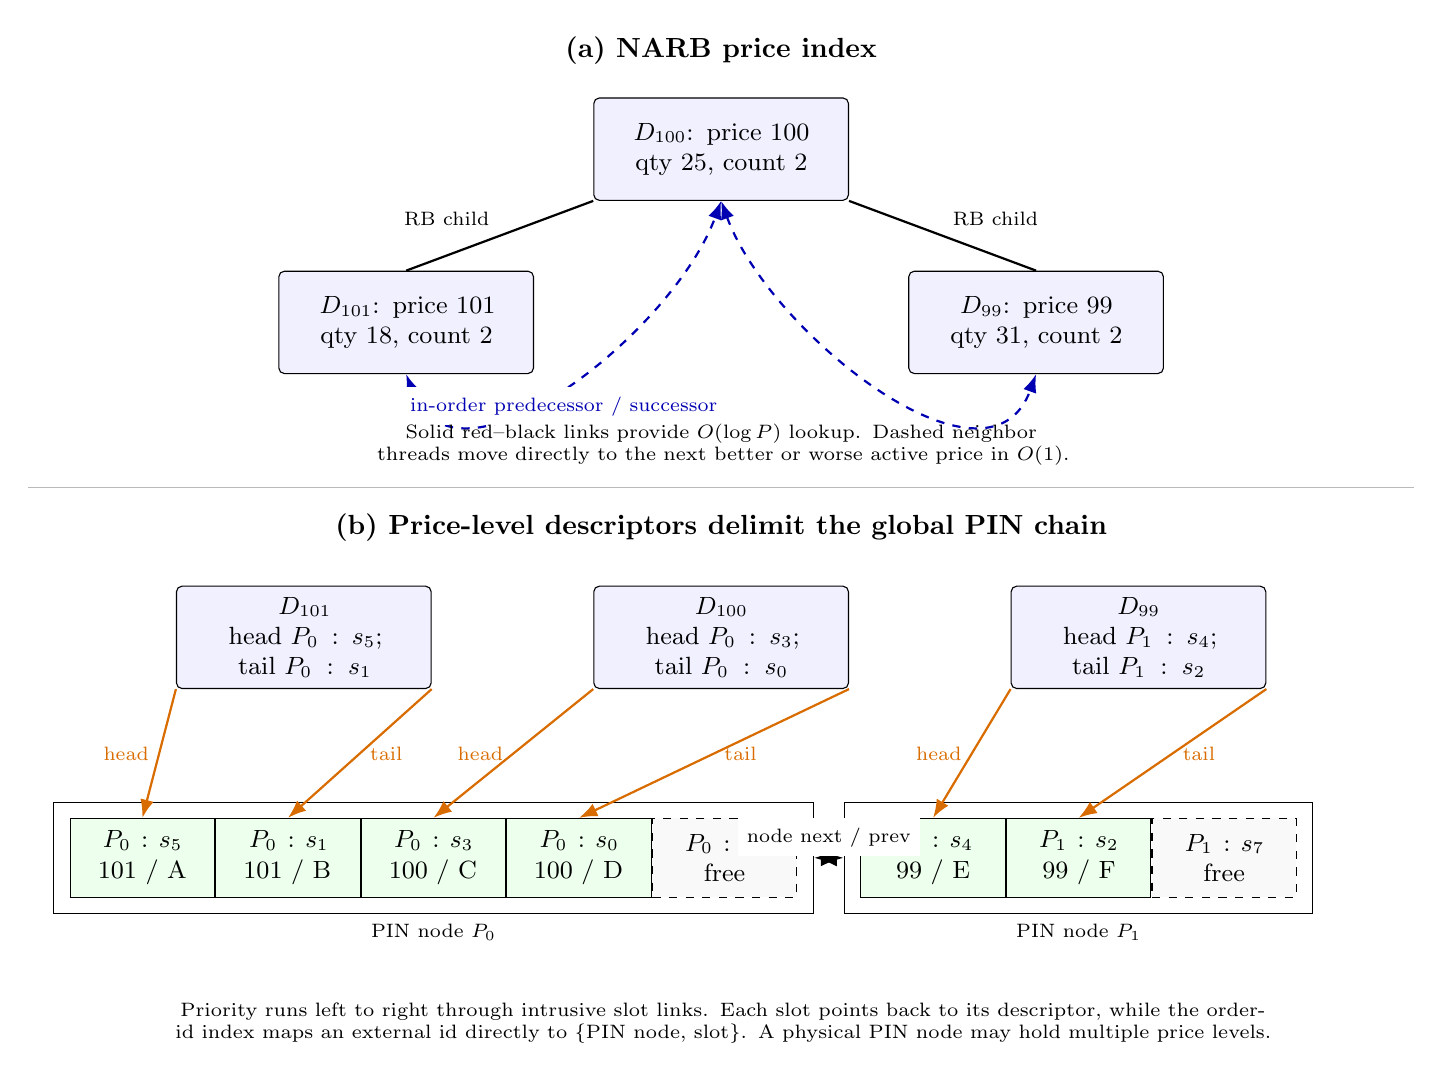
\begin{tikzpicture}[
  font=\small,
  desc/.style={draw,rounded corners=2pt,text width=30mm,minimum height=13mm,align=center,fill=blue!6},
  slot/.style={draw,text width=16mm,minimum height=10mm,align=center,fill=green!7},
  empty/.style={draw,dashed,text width=16mm,minimum height=10mm,align=center,fill=gray!5},
  treeedge/.style={thick},
  neighbor/.style={<->,>=Latex,dashed,blue!70!black,thick},
  ptr/.style={->,>=Latex,orange!85!black,thick},
  chain/.style={<->,>=Latex,very thick}
]
% Panel A: enough vertical space separates tree edges from neighbor threads.
\node[font=\bfseries] at (0,7.7) {(a) NARB price index};
\node[desc] (root) at (0,6.45) {$D_{100}$: price 100\\qty 25, count 2};
\node[desc] (high) at (-4.0,4.25) {$D_{101}$: price 101\\qty 18, count 2};
\node[desc] (low) at (4.0,4.25) {$D_{99}$: price 99\\qty 31, count 2};
\draw[treeedge] (root.south west) -- node[above left,font=\scriptsize]{RB child} (high.north);
\draw[treeedge] (root.south east) -- node[above right,font=\scriptsize]{RB child} (low.north);
\draw[neighbor] (high.south) to[out=-70,in=-110]
  node[below,font=\scriptsize,fill=white]{in-order predecessor / successor} (root.south);
\draw[neighbor] (root.south) to[out=-70,in=-110] (low.south);
\node[align=center,font=\scriptsize,text width=130mm] at (0,2.7)
  {Solid red--black links provide $O(\log P)$ lookup. Dashed neighbor threads
   move directly to the next better or worse active price in $O(1)$.};

\draw[gray!55] (-8.8,2.15) -- (8.8,2.15);

% Panel B: descriptors align above their ranges, keeping all six pointers separate.
\node[font=\bfseries] at (0,1.65) {(b) Price-level descriptors delimit the global PIN chain};
\node[desc] (d101) at (-5.3,0.25) {$D_{101}$\\head $P_0:s_5$; tail $P_0:s_1$};
\node[desc] (d100) at (0,0.25) {$D_{100}$\\head $P_0:s_3$; tail $P_0:s_0$};
\node[desc] (d99) at (5.3,0.25) {$D_{99}$\\head $P_1:s_4$; tail $P_1:s_2$};

\node[slot] (s5) at (-7.35,-2.55) {$P_0:s_5$\\101 / A};
\node[slot,right=0pt of s5] (s1) {$P_0:s_1$\\101 / B};
\node[slot,right=0pt of s1] (s3) {$P_0:s_3$\\100 / C};
\node[slot,right=0pt of s3] (s0) {$P_0:s_0$\\100 / D};
\node[empty,right=0pt of s0] (s6) {$P_0:s_6$\\free};
\node[draw,fit=(s5)(s6),inner sep=2mm,label={[font=\scriptsize]below:PIN node $P_0$}] (pin0) {};

\node[slot,right=8mm of s6] (t4) {$P_1:s_4$\\99 / E};
\node[slot,right=0pt of t4] (t2) {$P_1:s_2$\\99 / F};
\node[empty,right=0pt of t2] (t7) {$P_1:s_7$\\free};
\node[draw,fit=(t4)(t7),inner sep=2mm,label={[font=\scriptsize]below:PIN node $P_1$}] (pin1) {};
\draw[chain] (pin0.east) -- node[above,font=\scriptsize,fill=white]{node next / prev} (pin1.west);

\draw[ptr] (d101.south west) -- node[left,font=\scriptsize]{head} (s5.north);
\draw[ptr] (d101.south east) -- node[right,font=\scriptsize]{tail} (s1.north);
\draw[ptr] (d100.south west) -- node[left,font=\scriptsize]{head} (s3.north);
\draw[ptr] (d100.south east) -- node[right,font=\scriptsize]{tail} (s0.north);
\draw[ptr] (d99.south west) -- node[left,font=\scriptsize]{head} (t4.north);
\draw[ptr] (d99.south east) -- node[right,font=\scriptsize]{tail} (t2.north);

\node[align=center,font=\scriptsize,text width=155mm] at (0,-4.65)
  {Priority runs left to right through intrusive slot links. Each slot points
   back to its descriptor, while the order-id index maps an external id directly
   to \{PIN node, slot\}. A physical PIN node may hold multiple price levels.};
\end{tikzpicture}
\caption{Two complementary views of the architecture. The NARB Tree owns one
price-level descriptor per active price. Descriptor head/tail pointers identify
that price's logical range inside the global per-side PIN chain; order payloads
live only in stable PIN slots.}
\label{fig:global-pin-chain}
\end{figure*}


Every stored order carries a back-pointer to its price-level descriptor.  The
order-id index independently maps the public identifier to its current PIN node
and slot.  If a full-node cascade relocates a boundary order, the relocation
updates three kinds of reference: the id index, the moved order's descriptor
head/tail when the moved slot was a boundary, and the order's embedded level
back-pointer.  The logical sequence is preserved even though the payload changes
physical node and slot.  Cancellation uses the same references in reverse: it
updates descriptor aggregates and boundaries, unlinks the slot, removes an empty
PIN node if necessary, and removes the descriptor from the NARB Tree only when
the last order at that price has disappeared.

\subsection{Insertion into the PIN chain}

Once the NARB Tree has found or created the price-level descriptor, insertion
uses the descriptor to choose one exact global-priority anchor:
\begin{enumerate}
  \item If the side is empty, allocate one PIN node, append the order, and set
        both global chain endpoints to that node.
  \item If the price level already contains orders, its \texttt{\_tail} is the
        anchor.  The new order is inserted immediately after it, preserving FIFO
        time priority at that price.
  \item If this is a newly activated price, identify the immediately better
        descriptor from the NARB predecessor/successor threads.  Insert after
        that descriptor's tail.  If no better level exists, prepend at the global
        chain head because the new price is now best.
\end{enumerate}

The anchor is an \texttt{order\_loc}, not merely an order pointer, so it identifies
both a PIN node and a slot.  There are then three physical cases.  If the anchor
node has a free slot, \texttt{insert\_after} completes locally.  If the full
anchor is its node's tail, the new logical position is at the node boundary: the
order can be prepended to the next node, after first making room there, or placed
in a newly allocated tail node.  If the anchor is inside a full node, room must
be created in that same node before the local splice.

\paragraph{Bounded relocation cascade.}
\texttt{make\_room(X)} walks from node $X$ toward the global tail looking for a
node with one free slot.  The walk is capped at 16 node hops.  If every visited
node is full, a pooled node is inserted after the last visited node.  The
algorithm then walks the recorded path backward: move each source node's tail
order into the destination node's head.  Starting at the far end guarantees
that every destination already has room.  One free slot finally appears in
$X$.

Moving a source tail to the next node's head preserves global priority: that
order was immediately before the destination node's old head both before and
after relocation.  Each hop also updates the moved order's id-index entry and,
if necessary, its price descriptor's head or tail location.  Thus the cascade
moves at most one payload per visited node and has a configured upper bound
independent of total book size.  It is an insertion slow path, not part of normal
cancellation.

After physical placement, \texttt{place\_order} completes the cross-structure
transaction: write the order's descriptor back-pointer, initialize the
descriptor head if the level was empty, set its tail to the new location, insert
\texttt{order id -> order\_loc} into the hash index, add open quantity, and
increment the level count.  These references must agree before the next command
is processed.

\subsection{Direct cancellation}

Each side maintains an order-id index whose value contains the owning node,
slot, and price-level descriptor.  Cancellation is therefore:

\begin{center}
\texttt{id $\rightarrow$ location $\rightarrow$ unlink slot $\rightarrow$ recycle}
\end{center}

The index lookup is O(1) average and the slot unlink is O(1).  The level's
aggregate quantity and count are decremented at the same time.  If the node
becomes empty it is detached and returned to its pool; if the price level
becomes empty, the level is removed from the price tree.  The latter structural
event is not O(1), but it occurs only when the last order at a price disappears.

More precisely, cancellation executes the following sequence:
\begin{enumerate}
  \item Look up the id in the side's \texttt{unordered\_map}.  An absent id is
        already filled, cancelled, or unknown and leaves the structure unchanged.
  \item Read the slot's descriptor back-pointer, remove the id-index entry, and
        subtract the order's open quantity and one order from the descriptor.
  \item Compare the location with descriptor \texttt{\_head} and
        \texttt{\_tail}.  If it is a boundary, compute the replacement using
        \texttt{global\_next} or \texttt{global\_prev} \emph{before} unlinking,
        while the links are still valid.  If it was both boundaries, the price
        level has become empty.
  \item Unlink and recycle the PIN slot.  If the physical PIN node is now empty,
        detach it from the global node chain and return it to the PIN pool.
  \item Only when the price lost its final order, unlink its pred/succ price
        threads, update \texttt{best} when required, perform red--black deletion
        and fix-up, and return the descriptor to its pool.
\end{enumerate}
The common cancellation path therefore consists of one average-O(1) hash lookup,
aggregate/link updates, and a slot recycle.  Red--black work appears only on a
price-level transition, not for every cancelled order.

\subsection{NARB Tree: threaded price-level index}

The threaded price index is called the \emph{NARB Tree}---Neighbor-Aware
Red--Black Tree.  There is one \texttt{narb\_tree} for each side and separate
trees for parked stop orders.  Each red--black-tree node represents one active
price level and is called a \emph{price-level descriptor}; individual orders
remain in the PIN chain rather than becoming tree nodes.  A descriptor stores
the price, aggregate quantity, resting-order count, a location in the PIN chain,
normal red--black-tree links, and explicit predecessor/successor threads.
Known neighboring descriptors allow common near-touch insertions to splice at a
local position before the normal red--black rebalancing step.  The threads let
the matcher advance best-first
without restarting a root-to-leaf search after each exhausted level.  Bid and
ask template specializations reverse the price ordering while sharing the
implementation.

The red--black structure itself is ordered by numeric price: left children are
lower and right children higher.  Side semantics are applied only when deciding
which direction means ``better.''  Bids keep \texttt{\_best} at the maximum
descriptor and advance toward worse prices through \texttt{pred}; asks keep it
at the minimum and advance through \texttt{succ}.  This makes a best-first price
walk one pointer read per level without embedding side-dependent comparisons in
the iterator.

For an arbitrary price, \texttt{find\_neighbors} performs a normal O($\log P$)
red--black search while retaining the last lower and higher descriptors.  It
returns either an exact descriptor or the insertion pair
\{predecessor, successor\}.  Common near-touch cases bypass that traversal:
same as best, better than best, same as the immediate worse level, between best
and immediate worse, or adding the second level to a one-level book.

Given known neighbors, insertion does not search from the root a second time.
If the predecessor has no right child, the new descriptor becomes that right
child; otherwise it becomes the successor's left child.  The operation then
splices the descriptor into the pred/succ thread list, updates \texttt{\_best}
when the new node is the bid maximum or ask minimum, colors the node red, and
runs the standard red--black recolor/rotation fix-up toward the root.  The
neighbor knowledge removes discovery work; it does not remove the O($\log P$)
worst-case balancing path.

Deletion reverses those responsibilities in a safe order.  First remove the
descriptor from the pred/succ thread list and advance \texttt{\_best} if the
deleted node was best.  Next perform ordinary red--black transplant, successor
replacement for a two-child node, and black-height fix-up.  Finally recycle the
descriptor.  Unit tests expose \texttt{validate\_rb()}, which checks BST order,
a black root, no red/red edge, and equal black height on every root-to-leaf path.

\subsection{Memory pools and object lifetime}

PIN nodes and price-level descriptors use separate process-wide
\texttt{AllocatorPool<T>} instances.  A pool allocates memory in blocks rather
than asking the general-purpose heap for every object: PIN nodes use blocks of
128 objects, while descriptors use the pool's default block size of 1024.  Each
block is an array of aligned union chunks.  While occupied, a chunk contains a
properly constructed \texttt{T}; while free, the same bytes contain a pointer to
the next free chunk.

Allocation first pops the pool free list and constructs the object in place.  If
no recycled chunk exists, it takes the next unused chunk, growing the pool by a
block only when the high-water mark reaches current capacity.  Release calls the
object destructor and pushes the chunk onto the intrusive free list.  Blocks
themselves live until process shutdown, so growing the vector of block pointers
does not move any previously returned object.  PIN-node pointers, descriptor
pointers, tree links, and \texttt{order\_loc} references therefore remain stable.

Pooling contributes in three ways.  It amortizes expensive heap calls over many
objects, makes reuse a short free-list operation, and reduces fragmentation by
grouping equal-sized objects.  It also preserves the stable addresses required
by the cross-linked tree, descriptors, orders, and id index.  This benefit should
not be overstated: a block-growth event still allocates, and the unordered id
index has its own allocation behavior.  The current benchmarks do not isolate a
``pool-only'' speedup.  Rather, pooling removes per-node/per-descriptor allocator
traffic from the steady-state path and makes the surrounding direct-reference
design practical.

The pools contain no locks because the book is intentionally single-writer.
Adding concurrent writers would require synchronization or one pool per owner;
sharing these singleton pools across concurrently mutated books would violate
the present design assumption.

For readers following the implementation, the concepts map directly to source:
\begin{table}[h]
\centering
\caption{Architecture-to-source map.}
\scriptsize
\begin{tabular}{@{}ll@{}}
\toprule
Concept & Primary header \\
\midrule
PIN slots and node links & \texttt{data\_structures/pin\_node.h} \\
NARB Tree and global chain & \texttt{data\_structures/narb\_tree.h} \\
Price-level metadata & \texttt{price\_level\_descriptor.h} \\
Block/free-list allocator & \texttt{memory/memory\_pool.h} \\
Matching and order lifecycle & \texttt{book/matching\_book.h} \\
\bottomrule
\end{tabular}
\end{table}

The book owns no external order objects.  Trees hold resting and parked orders
by value, while callers interact using order identifiers.  Pools provide stable
storage for nodes and price descriptors; orders themselves live inline in PIN
slots rather than in separately allocated heap objects.

\subsection{Matching and lifecycle behavior}

\texttt{matching\_book<SIZE>} synchronously handles each command.
The new-order path crosses the best opposite prices, emits one trade per fill,
removes completed makers through the same direct index, and rests an eligible
residual.  IOC residuals are cancelled.  AON orders first check executable
quantity, while stop orders remain parked until the market price triggers them.
Canonical fill events are emitted synchronously through the id-based order listener.

The native book supports nuanced replace behavior, but the benchmark adapter
deliberately implements every modify as cancel plus reinsert.  This creates one
unambiguous semantic contract shared with \textit{Liquibook} and prevents a different
queue-priority rule from contaminating the comparison.

\subsection{Pull-based aggregate depth}

An earlier version eagerly maintained a separate depth tracker and an ordered
overflow map.  That design added work and allocation to every deep-book update.
The current order book instead treats the price trees as the source of truth.
Quantity and order count already live in each descriptor; \texttt{depth()} walks
the first \texttt{SIZE} threaded levels and materializes a passive snapshot only
when requested.  Thus depth publication is O(\texttt{SIZE}) per query but adds
almost no independent maintenance to the matching hot path.  Depth can also be
compiled as part of the single canonical configuration.

\subsection{System boundary}

The benchmark loads each adapter as a shared library.  Only fixed-layout C
structures cross the boundary: new order (32 bytes), cancel (16), modify (32),
tagged message (40), and report (64).  This avoids passing C++ standard-library
objects between modules with potentially different runtimes.

The harness sends commands, the adapter invokes its native order-book API, and reports
flow through a common transport drained on another core.  \textit{babobook} matches
synchronously, so its ABI-level \texttt{engine\_flush()} is a no-op; an asynchronous implementation
may return from message delivery earlier, but \texttt{engine\_flush()} must wait
for all work and reports and remains inside the timed region.

\section{Workload generation and scenarios}

The workload is synthetic and deterministic, not a replay of exchange order
identifiers.  It was published with Yoon's source benchmark~\cite{yoon2026} and calibrated to a
liquid U.S. equity.  Synthetic generation is useful here because public trade
and level-2 feeds generally do not reveal the complete add/cancel/replace
lifecycle or stable FIFO identity required to replay an order book.  The
generator produces those valid lifecycles explicitly while allowing one factor,
such as price-path volatility, to be controlled.

\subsection{Price path and placement}

The midpoint begins at \$167.52 and follows a driftless geometric Brownian
motion (GBM):
\begin{equation}
S_{t+\Delta t}=S_t\exp\!\left(-\tfrac12\sigma^2\Delta t+
\sigma\sqrt{\Delta t}Z_t\right),\quad Z_t\sim\mathcal N(0,1).
\end{equation}
The path is snapped to integer ticks of \$0.005 before reaching either order book;
matching itself performs no floating-point price comparison.

GBM is used here as a controllable environment generator, not as a claim that a
real security follows this equation exactly.  The parameter $\sigma$ controls
the instantaneous volatility scale, while $\Delta t$ determines how much of
that volatility is accumulated between generated orders.  For a non-static
scenario the generator chooses
\begin{equation}
\Delta t=\frac{(R/\sigma)^2}{N},
\end{equation}
where $R$ is the scenario's target swing and $N$ is the number of generated NEW
orders.  Consequently the per-step diffusion scale is
$\sigma\sqrt{\Delta t}=R/\sqrt{N}$.  Increasing $R$ spreads the same number of
orders across a wider price path; increasing $N$ creates more, smaller steps so
the total diffusion budget remains comparable.  The target swing controls the
scale of the stochastic path, not a guaranteed realized high-to-low percentage
for every seed.

Each passive order is placed $k+1$ ticks from the contemporaneous midpoint.
The level $k\in[0,799]$ is sampled from
\begin{equation}
w(k)=\frac{1}{(k+1)^{2.23}}+5\exp\!\left[-\tfrac12(k-8)^2\right].
\end{equation}
The power-law term produces a long tail, while the hump concentrates liquidity
several ticks behind the touch.  Quantities are uniform integers in $[1,100]$.

Buy prices are generated along the first half of the path and sell prices along
the second half.  A deterministic Fisher--Yates shuffle then interleaves both
sides into arrival order.  This is a construction technique that creates
crossing flow and a regime-dependent resting tail; it is not a behavioral claim
that real traders segregate sides by session half.

\subsection{Order lifecycle}

Each generated order receives a stable id.  Fifteen percent are IOC and receive
no later lifecycle message.  Of the remaining orders, 20\% receive a modify and
95\% later receive a cancel.  These probabilities overlap: a modified order can
subsequently be cancelled.  A modify increases quantity by one and, 80\% of the
time, moves one tick toward the market.  A small fraction of cancellations and
modifications are repeated after the order is gone, forcing both implementations to emit
the correct rejection.

Resting lifetime is exponentially distributed around a 0.431 ms median.  The
rate decreases with sampled depth $k$ as $\lambda_k=\lambda_0/\sqrt{1+k}$, so
near-touch orders churn quickly while deep orders remain longer.  All lifecycle
events are stably sorted by their synthetic timestamps.  One million NEW orders
therefore expand to roughly two million delivered commands rather than one
million independent operations.

\begin{table}[h]
\centering
\caption{Canonical workload parameters. Percentages are lifecycle decisions,
not mutually exclusive shares of all messages.}
\label{tab:params}
\scriptsize
\begin{tabular}{@{}lr@{}}
\toprule
Parameter & Value \\
\midrule
Start midpoint / tick & \$167.52 / \$0.005 \\
Placement distribution & power law + 8-tick hump \\
Quantity & uniform integer 1--100 \\
Cancel / modify / IOC & 95\% / 20\% / 15\% \\
Median resting lifetime & 0.431 ms \\
Duplicate cancel / stale modify & 2\% / 2\% \\
NEW orders / canonical seed & 1,000,000 / 23 \\
\bottomrule
\end{tabular}
\end{table}

\subsection{Scenario matrix}

Only the GBM volatility and target swing change across scenarios
(Table~\ref{tab:scenarios}).  \textit{Normal} is the representative simulated
workload.  \textit{Static} fixes the midpoint and creates the deepest per-price
queues, making it a cancellation-complexity stress test.  The wider paths test
whether larger price trees and working sets cause abrupt degradation.

The five environments answer different questions rather than serving as five
attempts to find a favorable number:
\begin{itemize}
  \item \textbf{Static} sets $\sigma=R=0$, so the midpoint never moves.  Orders
        repeatedly land around the same prices and create long FIFO queues.  It
        isolates arbitrary-cancel cost and is intentionally harsher than normal
        trading for Liquibook's scan-based cancel path.
  \item \textbf{Normal} uses $\sigma=0.15$ and $R=2\%$.  Prices drift over a
        relatively narrow range, so the book experiences routine matching,
        cancellation, modification, and a moderate number of active levels.  It
        is the representative scenario behind the headline comparison.
  \item \textbf{Swing-25} keeps the high-volatility setting $\sigma=0.50$ but
        raises $R$ to 25\%.  Orders spread over many more ticks, expanding the
        price tree and its cache footprint.
  \item \textbf{Swing-40} raises the target to 40\%, representing a more severe
        stressed session.  It checks whether throughput degrades smoothly as
        the active price range widens.
  \item \textbf{Flash-crash} uses the same stochastic model with $R=60\%$.  It
        represents an extreme dislocation and the widest working set.  The name
        describes the stress regime; the generator is not a replay of a specific
        historical crash and does not force a deterministic downward path.
\end{itemize}

Testing every implementation on every environment separates two possible
sources of speed: long per-price queues in a narrow market and a large ordered
price index in a volatile market.  Static emphasizes queue occupancy; the swing
scenarios emphasize tree width and cache working set; normal combines the common
operations without maximizing either extreme.  A design that wins only static
has demonstrated a useful cancel optimization, but not yet robust performance
under changing prices.  The cross-scenario comparison is therefore part of the
claim, not supplementary decoration.

\begin{table}[h]
\centering
\caption{Workload scenarios and their experimental purpose.}
\label{tab:scenarios}
\scriptsize
\begin{tabular}{@{}lrrp{0.40\columnwidth}@{}}
\toprule
Scenario & $\sigma$ & Swing & Purpose \\
\midrule
Static & 0.00 & 0\% & deep-queue cancel stress \\
Normal & 0.15 & 2\% & representative routine flow \\
Swing-25 & 0.50 & 25\% & high-volatility wide book \\
Swing-40 & 0.50 & 40\% & severely stressed book \\
Flash-crash & 0.50 & 60\% & extreme dislocation \\
\bottomrule
\end{tabular}
\end{table}

For portability, distributions are implemented directly over
\texttt{std::mt19937}: Box--Muller for normal draws, inverse exponential
sampling, a precomputed placement CDF, and explicit Fisher--Yates shuffling.
The generator disables FMA contraction and LTO.  Transcendental math can still
differ in the last bit across platform math libraries, so correctness references
are regenerated with the trusted baseline on the machine being measured.
\texttt{-ffast-math} is forbidden because it can change the workload itself.

\section{Correctness before speed}
\label{sec:correctness}

A throughput result is meaningless if an order book skips state transitions,
drops reports, or implements different matching semantics.  The project uses
three complementary checks.

First, GoogleTest exercises babobook directly: bid and ask insertion,
partial and multi-level fills, maker-price execution, cancellation, rejection,
replace behavior, IOC/FOK, AON, stops, market price, depth ordering and
aggregation, and the canonical fill-event stream.  The vendored upstream \textit{Liquibook} tests remain a
frozen baseline.

Second, the harness hashes the entire 64-byte report stream.  References are
generated by the trusted baseline for each scenario.  \textit{babobook} must reproduce
the same OrderAck, Trade, CancelAck, ModifyAck, CancelReject, and ModifyReject
records in the same order, including identifiers, prices, and quantities.  A
SHA-256 match is stronger than comparing trade counts, which can hide different
fills or missing rejection paths.

Third, a malicious or accidentally optimized implementation could replay known reports
without maintaining a book.  Audit mode prevents this by stopping at 64
unpredictable replay indices and comparing best bid, best ask, and depth at
selected prices with a live trusted baseline.  Optional prebuild and batch APIs
are subject to the same state contract and cannot net future messages against
earlier ones.

Hash equality is not a formal proof for all possible inputs.  It establishes
observational equivalence for the evaluated stream under a shared semantic
contract.  Unit tests, multiple scenarios, stale requests, and state probes cover
different failure modes and are intentionally retained alongside the hash.

\section{Evaluation methodology}

The evaluation uses two complementary measurement paths with deliberately
distinct jobs, and it is important not to conflate them.

\emph{Correctness is certified by the harness.}  The harness loads each engine as
a shared library across the C ABI, replays the workload one message at a time,
drains the complete 64-byte report stream over the SPSC transport on an adjacent
core, hashes it with SHA-256, and compares the result against the trusted
reference; it additionally runs the state audit at unpredictable replay indices
(Section~\ref{sec:correctness}).  The harness therefore exercises delivery,
matching, report production, transport, and the final flush, and it is the
component that proves the measured engine emits byte-identical output rather than
skipping work.

\emph{Throughput is measured by the standalone perf binaries.}  These link each
order book directly---no adapter, no shared-library boundary, and no report
transport---pin to an isolated core, raise scheduling priority, and replay the
same deterministic workload, reporting the peak of $N$ repetitions.  Isolating
throughput this way keeps the reported figure free of report-emission and
cross-module transport overhead, so it reflects the matching core itself; the
harness independently guarantees that the core being timed is correct.  Every
throughput number in this paper comes from the perf path; every correctness and
audit verdict comes from the harness path.

Release builds use C++20, O3/native ISA tuning and loop unrolling where the GNU
driver is used, plus LTO when supported.  Both order books receive the same binary
workload through the same C ABI and perform the same modify-as-reinsert semantics.

\paragraph{Frequency stability.}  Absolute throughput tracks the core's operating
frequency, which the hardware scales with thermal and power state.  On the mobile
parts used here the base-to-boost range is roughly $2\times$ (about $2.0$ vs.\
$4.5$~GHz on the Ryzen~7~7730U), so an unconstrained core reports the \emph{same}
workload at ${\approx}8$ or ${\approx}17$~M~messages/s depending only on how long
it has been under load: short boost bursts are not sustainable across a
multi-minute sweep and decay to the base clock as the die heats.  We therefore
disable CPU boost for measurement and record every cell at the fixed base clock
(Windows \texttt{powercfg PERFBOOSTMODE=0} on the AMD host; the analogous
processor-power policy elsewhere), retaining core pinning and elevated priority as
above.  A fixed clock does not change the \emph{speedup}---a ratio measured at a
common frequency---but it removes a systematic bias: the two engines are timed
back to back within each cell, and because a slower engine's longer run would
otherwise accumulate more thermal throttling than a faster engine's, a
boost-enabled measurement inflates the ratio toward the faster engine.  Apple
Silicon exposes neither core pinning nor a boost lock, so those hosts are measured
at stock frequency policy and reported as a distinct, harder measurement
condition.

The final paper will report CPU, topology, memory, operating system, compiler,
build flags, git revision, core affinity, priority status, processor frequency
policy (CPU boost disabled, fixed base clock), warm-up policy, repetitions,
aggregation statistic, and run-to-run dispersion.  Correctness and
audit status accompany every reported comparison.  The benchmark must be rerun
after the recent pull-based depth change; old saved results are retained only as
development evidence, not silently promoted to final measurements.

\section{Results}

Table~\ref{tab:results} is deliberately structured around the final clean run.
The checked-in pre-redesign harness result measured 4.20 Mmsg/s for \textit{babobook} and
2.71 Mmsg/s for \textit{Liquibook} on \textit{normal} (1.55$\times$), while
\textit{static} measured 4.78 versus 0.06 Mmsg/s (79.7$\times$); all scenario
hashes passed.  Those numbers establish the static mechanism but do not yet
support the proposed 4$\times$ representative headline.  The cells below will
be replaced only by the post-rebuild core-pinned measurement matrix, with each
row's correctness certified by the harness as described in
Section~\ref{sec:correctness}.

\begin{table}[h]
\centering
\caption{Core-pinned perf throughput (direct-linked engine, no adapter or report
transport). Every row is independently certified by the harness's SHA-256
report-stream match; values await the clean canonical run.}
\label{tab:results}
\scriptsize
\begin{tabular}{@{}lrrrl@{}}
\toprule
Scenario & \textit{Liquibook} & \textit{babobook} & Speedup & Correct \\
 & \multicolumn{2}{c}{M messages/s} & & \\
\midrule
Static & \todo{L} & \todo{B} & \todo{x} & PASS \\
Normal & \todo{L} & \todo{B} & \todo{x} & PASS \\
Swing-25 & \todo{L} & \todo{B} & \todo{x} & PASS \\
Swing-40 & \todo{L} & \todo{B} & \todo{x} & PASS \\
Flash-crash & \todo{L} & \todo{B} & \todo{x} & PASS \\
\bottomrule
\end{tabular}
\end{table}

The most important explanatory result will be a scaling curve: cancellation
throughput versus resting orders per price (or total resting-book size).  A
single static endpoint shows a large ratio, but the curve can test the causal
claim directly.  If \textit{Liquibook}'s scan is dominant, its throughput should fall as
queues deepen; \textit{babobook}'s direct path should remain flatter until cache capacity or
index size becomes the limiting factor.

A separate payload-size experiment runs the complete normal scenario from 1K,
10K, 100K, 1M, and 10M generated NEW orders, with a 100M point available as an
explicit huge run.  It records delivered lifecycle messages, throughput for both
implementations, speedup, and equality of their freshly computed report hashes,
then emits CSV, Markdown, and an SVG graph.  This curve measures warm-up and
sustained-throughput behavior as replay duration grows; it must not be confused
with data-structure scaling, because the canonical 95\% cancellation lifecycle
keeps the live resting book far smaller than the cumulative input payload.  The
current materializing harness makes 100M NEW orders a multi-gigabyte workload
with potentially tens of gigabytes of peak memory, so that point is reported
only on hardware capable of completing it without paging.

Pull-based depth is part of the single canonical configuration and is not
reported as a separate benchmark dimension.  The PIN-capacity sweep remains a
documented robustness check; it produced no meaningful difference across the
tested capacities.

\section{Threats to validity}

The workload is calibrated synthetic traffic, not raw market-by-order data.
Its lifecycle ratios and path construction may differ from a particular venue.
The static workload is intentionally adversarial and must not be presented as a
normal session.  A future real-data-calibrated workload can use recorded public
midpoint, spread, depth, and update distributions, but a level-2 feed cannot be
truthfully converted into original FIFO order identities without inventing
events.

The principal comparison is against one version of one baseline.  \textit{Liquibook}'s
linear cancel lookup is an implementation choice, not an unavoidable property
of every tree-of-lists book; adding a direct id index would close much of the
static gap.  Hardware, compiler, allocator, core isolation, power policy, and
thermal state can all affect absolute throughput.  The adapter boundary reduces
semantic differences but cannot make two order books' internal feature sets
identical.

Finally, the theoretical PIN and neighbor-aware-tree direction is attributed to
Yoon~\cite{yoon2026}, whose paper states that related implementations are covered by a patent
portfolio.  This report claims independent implementation effort, not ownership
of that theory or a legal conclusion about patent scope.  The C-ABI harness and
workload infrastructure were adapted from Flash One's public benchmark
repository~\cite{flashbenchmark}; Liquibook is the separately licensed baseline,
and Rigtorp's SPSCQueue carries reports from the producer to the drainer
thread~\cite{rigtorp}.  These components are not presented as original babobook
code.  Their copyright notices, license texts, provenance, and local locations
are recorded in the repository's \texttt{THIRD\_PARTY\_NOTICES.md} and adjacent
upstream license files.

\section{Reproducing and extending the benchmark}

After a Release configure, the repository builds both order books, adapters, perf
binaries, and two test executables.  The reproducible sequence is:
\begin{enumerate}
  \item build the canonical configuration;
  \item run all unit tests;
  \item regenerate the five workloads and trusted \textit{Liquibook} hashes locally;
  \item require \textit{babobook} to reproduce every hash;
  \item run the five-scenario comparison with fixed repetition policy; and
  \item run audit mode once as a pass/fail state certification.
\end{enumerate}
The repository supplies equivalent PowerShell and shell scripts.  CSV, Markdown,
and per-run JSON outputs are retained with the environment metadata used by the
paper.

For cross-machine collection, \texttt{scripts/run\_portable\_perf.py} is the
single platform-neutral runner behind PowerShell and shell wrappers.  By default
it executes \texttt{babo\_perf} and \texttt{liqui\_perf} across all five market
states with one warmup and 100 measured replays per state.  Each run creates a
shareable ZIP containing a human-readable table, CSV and JSON, raw output,
operating-system and CPU information, compiler identity and flags, CMake cache
hash, git revision and dirty status, binary SHA-256 hashes, and a manifest.  This
makes results from Windows, macOS, and Linux---and from GCC, Clang, Apple Clang,
or MSVC-style builds---comparable without manually transcribing terminal output.
The static Liquibook case can make the full matrix an overnight run, so execution
order and elapsed time remain visible in the generated artifacts.

Another order book can start from \texttt{benchmark/adapters/template\_adapter.h.cpp}
and implement initialization, new, cancel, modify, flush, and best/depth query
functions.  It may optionally provide its own transport, prebuild representation,
or batch entry point, but must honor the documented anti-cheat contract.  The
correct order of evaluation is strict: establish the full report hash, pass live
state audit, and only then compare throughput.  A published external result
should include the order-book revision, adapter source, hardware, compiler, flags,
scenario parameters, repetitions, dispersion, hashes, and audit verdict.

The workload-size graph is generated on Windows with
\texttt{scripts/compare\_payload\_scaling.ps1}.  Its default run covers 1K through
10M NEW orders; \texttt{-Include100M} opts into the resource-intensive final
point.  The script compares the computed hashes from Liquibook and babobook
directly because the shipped reference file intentionally covers the canonical
1M workload rather than every possible payload size.

\section{Conclusion}

The project demonstrates a general low-latency lesson: performance followed from
matching the data structure to the dominant operation.  A direct id-to-slot map
removed a depth-dependent search from cancellation; stable inline slots combined
locality with arbitrary erase; threaded price levels avoided repeated ordered
search during matching; and pull-based depth removed redundant hot-path state.
The static scenario exposes that mechanism dramatically, while the representative
scenario and volatility sweep test whether the design remains useful outside its
best case.

Equally important, the benchmark treats correctness as a prerequisite rather
than an afterthought.  Identical inputs, a C ABI, complete report hashing, and
unpredictable state probes make it harder to win by doing less work.  The final
claim will be the strongest result that survives the clean, reproducible run---not
the largest number available during development.

\begin{thebibliography}{9}
\small
\bibitem{yoon2026}
J. Yoon, ``The World's Fastest Matching Engine Algorithm,''
\textit{arXiv:2606.01183v3}, 2026,
\url{https://arxiv.org/abs/2606.01183}.

\bibitem{liquibook}
E. Newhuis and contributors, ``Liquibook: Modern C++ order matching engine,''
GitHub repository, source, README, and license,
\url{https://github.com/enewhuis/liquibook}, accessed July 11, 2026.

\bibitem{gould2013}
M. D. Gould et al., ``Limit order books,'' \textit{Quantitative Finance},
vol. 13, no. 11, 2013.

\bibitem{cont2010}
R. Cont, S. Stoikov, and R. Talreja, ``A stochastic model for order book
dynamics,'' \textit{Operations Research}, vol. 58, no. 3, 2010.

\bibitem{rigtorp}
E. Rigtorp, ``SPSCQueue: A bounded single-producer single-consumer queue,''
GitHub repository, \url{https://github.com/rigtorp/SPSCQueue}.

\bibitem{flashbenchmark}
Flash One Technologies LLC, ``Matching Engine Algorithm Performance
Challenge,'' GitHub repository,
\url{https://github.com/flash1-dev/matching-engine-benchmark}.
\end{thebibliography}

\end{document}
